\documentclass[11pt]{article}
\usepackage[utf8]{inputenc}
\usepackage[T1]{fontenc}
\usepackage{lmodern}
\usepackage[margin=1in]{geometry}
\usepackage{amsmath,amssymb}
\usepackage{booktabs}
\usepackage{multirow}
\usepackage{algorithm}
\usepackage[noend]{algpseudocode}
\usepackage{pgfplots}
\pgfplotsset{compat=1.16}
\usepackage[numbers,sort&compress]{natbib}
\usepackage{microtype}
\usepackage{xcolor}
\usepackage[colorlinks=true,linkcolor=blue!50!black,citecolor=blue!50!black,urlcolor=blue!50!black]{hyperref}

% Every measured number in this paper is generated from paper/data/ by
% paper/gen_tables.js; nothing below is typed in by hand.
\newcommand{\Commit}{657ed2d80f3c}
\newcommand{\RepoDate}{2026-10-27}
\newcommand{\NodeVersion}{v22.23.2}
\newcommand{\CPU}{Apple M3 Pro}
\newcommand{\Platform}{darwin, arm64}
\newcommand{\lookup}[1]{\ifcsname #1\endcsname\csname #1\endcsname\else\textbf{??#1}\fi}
\newcommand{\rt}[3]{\lookup{rt@#1@#2@#3}}
\newcommand{\ts}[2]{\lookup{ts@#1@#2}}
\newcommand{\val}[1]{\lookup{v@#1}}
\expandafter\def\csname v@hkInstances\endcsname{26}
\expandafter\def\csname v@hkHitsAll\endcsname{26/26}
\expandafter\def\csname v@hk18\endcsname{54\,ms--72\,ms}
\expandafter\def\csname v@hk20\endcsname{247\,ms--289\,ms}
\expandafter\def\csname v@hk22\endcsname{1.21\,s--1.46\,s}
\expandafter\def\csname rt@greedy@20@ms\endcsname{3\,\textmu s}
\expandafter\def\csname rt@greedy@20@gap\endcsname{+14.03\%}
\expandafter\def\csname rt@greedy@50@ms\endcsname{6\,\textmu s}
\expandafter\def\csname rt@greedy@50@gap\endcsname{+27.72\%}
\expandafter\def\csname rt@greedy@100@ms\endcsname{13\,\textmu s}
\expandafter\def\csname rt@greedy@100@gap\endcsname{+31.90\%}
\expandafter\def\csname rt@greedy@200@ms\endcsname{24\,\textmu s}
\expandafter\def\csname rt@greedy@200@gap\endcsname{+31.05\%}
\expandafter\def\csname rt@greedy@400@ms\endcsname{50\,\textmu s}
\expandafter\def\csname rt@greedy@400@gap\endcsname{+26.46\%}
\expandafter\def\csname rt@beam@20@ms\endcsname{204\,\textmu s}
\expandafter\def\csname rt@beam@20@gap\endcsname{+14.94\%}
\expandafter\def\csname rt@beam@50@ms\endcsname{496\,\textmu s}
\expandafter\def\csname rt@beam@50@gap\endcsname{+32.13\%}
\expandafter\def\csname rt@beam@100@ms\endcsname{2.1\,ms}
\expandafter\def\csname rt@beam@100@gap\endcsname{+32.43\%}
\expandafter\def\csname rt@beam@200@ms\endcsname{9.4\,ms}
\expandafter\def\csname rt@beam@200@gap\endcsname{+37.64\%}
\expandafter\def\csname rt@beam@400@ms\endcsname{43\,ms}
\expandafter\def\csname rt@beam@400@gap\endcsname{+38.88\%}
\expandafter\def\csname rt@tuned@20@ms\endcsname{1.1\,ms}
\expandafter\def\csname rt@tuned@20@gap\endcsname{0.00\%}
\expandafter\def\csname rt@tuned@50@ms\endcsname{5.9\,ms}
\expandafter\def\csname rt@tuned@50@gap\endcsname{+0.04\%}
\expandafter\def\csname rt@tuned@100@ms\endcsname{43\,ms}
\expandafter\def\csname rt@tuned@100@gap\endcsname{+0.69\%}
\expandafter\def\csname rt@tuned@200@ms\endcsname{441\,ms}
\expandafter\def\csname rt@tuned@200@gap\endcsname{+1.54\%}
\expandafter\def\csname rt@tuned@400@ms\endcsname{4.10\,s}
\expandafter\def\csname rt@tuned@400@gap\endcsname{+2.22\%}
\expandafter\def\csname rt@nature@20@ms\endcsname{11\,ms}
\expandafter\def\csname rt@nature@20@gap\endcsname{0.00\%}
\expandafter\def\csname rt@nature@50@ms\endcsname{64\,ms}
\expandafter\def\csname rt@nature@50@gap\endcsname{+0.07\%}
\expandafter\def\csname rt@nature@100@ms\endcsname{85\,ms}
\expandafter\def\csname rt@nature@100@gap\endcsname{+0.69\%}
\expandafter\def\csname rt@nature@200@ms\endcsname{178\,ms}
\expandafter\def\csname rt@nature@200@gap\endcsname{+3.40\%}
\expandafter\def\csname rt@nature@400@ms\endcsname{553\,ms}
\expandafter\def\csname rt@nature@400@gap\endcsname{+35.39\%}
\expandafter\def\csname rt@christofides@20@ms\endcsname{220\,\textmu s}
\expandafter\def\csname rt@christofides@20@gap\endcsname{+10.50\%}
\expandafter\def\csname rt@christofides@50@ms\endcsname{613\,\textmu s}
\expandafter\def\csname rt@christofides@50@gap\endcsname{+10.07\%}
\expandafter\def\csname rt@christofides@100@ms\endcsname{1.1\,ms}
\expandafter\def\csname rt@christofides@100@gap\endcsname{+13.07\%}
\expandafter\def\csname rt@christofides@200@ms\endcsname{11\,ms}
\expandafter\def\csname rt@christofides@200@gap\endcsname{+13.49\%}
\expandafter\def\csname rt@christofides@400@ms\endcsname{27\,ms}
\expandafter\def\csname rt@christofides@400@gap\endcsname{+13.03\%}
\expandafter\def\csname rt@lkh@20@ms\endcsname{13\,ms}
\expandafter\def\csname rt@lkh@20@gap\endcsname{0.00\%}
\expandafter\def\csname rt@lkh@50@ms\endcsname{50\,ms}
\expandafter\def\csname rt@lkh@50@gap\endcsname{0.00\%}
\expandafter\def\csname rt@lkh@100@ms\endcsname{97\,ms}
\expandafter\def\csname rt@lkh@100@gap\endcsname{0.00\%}
\expandafter\def\csname rt@lkh@200@ms\endcsname{672\,ms}
\expandafter\def\csname rt@lkh@200@gap\endcsname{+0.11\%}
\expandafter\def\csname rt@lkh@400@ms\endcsname{1.40\,s}
\expandafter\def\csname rt@lkh@400@gap\endcsname{+0.37\%}
\expandafter\def\csname rt@bgma-low@20@ms\endcsname{1.3\,ms}
\expandafter\def\csname rt@bgma-low@20@gap\endcsname{0.00\%}
\expandafter\def\csname rt@bgma-low@50@ms\endcsname{4.1\,ms}
\expandafter\def\csname rt@bgma-low@50@gap\endcsname{+0.12\%}
\expandafter\def\csname rt@bgma-low@100@ms\endcsname{12\,ms}
\expandafter\def\csname rt@bgma-low@100@gap\endcsname{+0.52\%}
\expandafter\def\csname rt@bgma-low@200@ms\endcsname{83\,ms}
\expandafter\def\csname rt@bgma-low@200@gap\endcsname{+1.70\%}
\expandafter\def\csname rt@bgma-low@400@ms\endcsname{622\,ms}
\expandafter\def\csname rt@bgma-low@400@gap\endcsname{+2.22\%}
\expandafter\def\csname rt@bgma-mid@20@ms\endcsname{5.0\,ms}
\expandafter\def\csname rt@bgma-mid@20@gap\endcsname{0.00\%}
\expandafter\def\csname rt@bgma-mid@50@ms\endcsname{14\,ms}
\expandafter\def\csname rt@bgma-mid@50@gap\endcsname{0.00\%}
\expandafter\def\csname rt@bgma-mid@100@ms\endcsname{37\,ms}
\expandafter\def\csname rt@bgma-mid@100@gap\endcsname{+0.03\%}
\expandafter\def\csname rt@bgma-mid@200@ms\endcsname{222\,ms}
\expandafter\def\csname rt@bgma-mid@200@gap\endcsname{+0.69\%}
\expandafter\def\csname rt@bgma-mid@400@ms\endcsname{1.95\,s}
\expandafter\def\csname rt@bgma-mid@400@gap\endcsname{+1.13\%}
\expandafter\def\csname rt@bgma-high@20@ms\endcsname{9.6\,ms}
\expandafter\def\csname rt@bgma-high@20@gap\endcsname{0.00\%}
\expandafter\def\csname rt@bgma-high@50@ms\endcsname{31\,ms}
\expandafter\def\csname rt@bgma-high@50@gap\endcsname{0.00\%}
\expandafter\def\csname rt@bgma-high@100@ms\endcsname{84\,ms}
\expandafter\def\csname rt@bgma-high@100@gap\endcsname{+0.02\%}
\expandafter\def\csname rt@bgma-high@200@ms\endcsname{625\,ms}
\expandafter\def\csname rt@bgma-high@200@gap\endcsname{+0.31\%}
\expandafter\def\csname rt@bgma-high@400@ms\endcsname{6.37\,s}
\expandafter\def\csname rt@bgma-high@400@gap\endcsname{+0.60\%}
\expandafter\def\csname rt@bgma-xhigh@20@ms\endcsname{16\,ms}
\expandafter\def\csname rt@bgma-xhigh@20@gap\endcsname{0.00\%}
\expandafter\def\csname rt@bgma-xhigh@50@ms\endcsname{52\,ms}
\expandafter\def\csname rt@bgma-xhigh@50@gap\endcsname{0.00\%}
\expandafter\def\csname rt@bgma-xhigh@100@ms\endcsname{212\,ms}
\expandafter\def\csname rt@bgma-xhigh@100@gap\endcsname{0.00\%}
\expandafter\def\csname rt@bgma-xhigh@200@ms\endcsname{1.81\,s}
\expandafter\def\csname rt@bgma-xhigh@200@gap\endcsname{+0.02\%}
\expandafter\def\csname rt@bgma-xhigh@400@ms\endcsname{15.0\,s}
\expandafter\def\csname rt@bgma-xhigh@400@gap\endcsname{+0.12\%}
\expandafter\def\csname rt@bgma-max@20@ms\endcsname{65\,ms}
\expandafter\def\csname rt@bgma-max@20@gap\endcsname{0.00\%}
\expandafter\def\csname rt@bgma-max@50@ms\endcsname{203\,ms}
\expandafter\def\csname rt@bgma-max@50@gap\endcsname{0.00\%}
\expandafter\def\csname rt@bgma-max@100@ms\endcsname{676\,ms}
\expandafter\def\csname rt@bgma-max@100@gap\endcsname{0.00\%}
\expandafter\def\csname rt@bgma-max@200@ms\endcsname{5.46\,s}
\expandafter\def\csname rt@bgma-max@200@gap\endcsname{+0.01\%}
\expandafter\def\csname rt@bgma-max@400@ms\endcsname{48.6\,s}
\expandafter\def\csname rt@bgma-max@400@gap\endcsname{+0.00\%}
\expandafter\def\csname rt@bound@20@ms\endcsname{96\,\textmu s}
\expandafter\def\csname rt@bound@50@ms\endcsname{3.5\,ms}
\expandafter\def\csname rt@bound@100@ms\endcsname{15\,ms}
\expandafter\def\csname rt@bound@200@ms\endcsname{66\,ms}
\expandafter\def\csname rt@bound@400@ms\endcsname{263\,ms}
\expandafter\def\csname rt@exact@20@ms\endcsname{299\,ms}
\expandafter\def\csname v@ratios20\endcsname{3.8, 1.9, 1.7, 4.0}
\expandafter\def\csname v@ratios50\endcsname{3.5, 2.2, 1.7, 3.9}
\expandafter\def\csname v@ratios100\endcsname{3.2, 2.3, 2.5, 3.2}
\expandafter\def\csname v@ratios200\endcsname{2.7, 2.8, 2.9, 3.0}
\expandafter\def\csname v@ratios400\endcsname{3.1, 3.3, 2.4, 3.2}
\expandafter\def\csname v@lowVsLkTime400\endcsname{0.44}
\expandafter\def\csname v@xhighVsLk400\endcsname{11}
\expandafter\def\csname v@maxVsLk400\endcsname{35}
\expandafter\def\csname v@tunedVsLow400\endcsname{6.6}
\expandafter\def\csname v@exp@bgma-low\endcsname{2.9}
\expandafter\def\csname v@exp@bgma-max\endcsname{3.1}
\expandafter\def\csname v@exp@lkh\endcsname{1.9}
\expandafter\def\csname v@chrVsLow\endcsname{6--86}
\expandafter\def\csname v@chrRange\endcsname{+10.07\% to +13.49\%}
\expandafter\def\csname v@expAll@bgma-low\endcsname{2.1}
\expandafter\def\csname v@expAll@bgma-max\endcsname{2.2}
\expandafter\def\csname v@expAll@lkh\endcsname{1.6}
\expandafter\def\csname ts@eil51@name\endcsname{eil51}
\expandafter\def\csname ts@eil51@n\endcsname{51}
\expandafter\def\csname ts@eil51@opt\endcsname{426}
\expandafter\def\csname ts@eil51@seeds\endcsname{10}
\expandafter\def\csname ts@eil51@maxHits\endcsname{9}
\expandafter\def\csname ts@eil51@maxBest\endcsname{426}
\expandafter\def\csname ts@eil51@maxMedGap\endcsname{0.000\%}
\expandafter\def\csname ts@eil51@maxWorstGap\endcsname{+0.235\%}
\expandafter\def\csname ts@eil51@maxSerial\endcsname{352\,ms}
\expandafter\def\csname ts@eil51@maxWall\endcsname{129\,ms}
\expandafter\def\csname ts@eil51@xhighHits\endcsname{9}
\expandafter\def\csname ts@eil51@lkHits\endcsname{1}
\expandafter\def\csname ts@eil51@lkBest\endcsname{426}
\expandafter\def\csname ts@eil51@lkMedGap\endcsname{+0.235\%}
\expandafter\def\csname ts@eil51@lkMs\endcsname{19\,ms}
\expandafter\def\csname ts@eil51@lkTotal\endcsname{196\,ms}
\expandafter\def\csname ts@eil51@boundBelow\endcsname{+0.823\%}
\expandafter\def\csname ts@eil51@boundGap\endcsname{+0.829\%}
\expandafter\def\csname ts@eil51@maxBestGap\endcsname{0.000\%}
\expandafter\def\csname ts@eil51@armXhigh\endcsname{0.00\%}
\expandafter\def\csname ts@eil51@armMax\endcsname{0.00\% and +0.23\%}
\expandafter\def\csname ts@eil51@wallS1\endcsname{170\,ms}
\expandafter\def\csname ts@eil51@serialS1\endcsname{377\,ms}
\expandafter\def\csname ts@eil51@lkBestGap\endcsname{0.000\%}
\expandafter\def\csname ts@berlin52@name\endcsname{berlin52}
\expandafter\def\csname ts@berlin52@n\endcsname{52}
\expandafter\def\csname ts@berlin52@opt\endcsname{7542}
\expandafter\def\csname ts@berlin52@seeds\endcsname{10}
\expandafter\def\csname ts@berlin52@maxHits\endcsname{10}
\expandafter\def\csname ts@berlin52@maxBest\endcsname{7542}
\expandafter\def\csname ts@berlin52@maxMedGap\endcsname{0.000\%}
\expandafter\def\csname ts@berlin52@maxWorstGap\endcsname{0.000\%}
\expandafter\def\csname ts@berlin52@maxSerial\endcsname{385\,ms}
\expandafter\def\csname ts@berlin52@maxWall\endcsname{142\,ms}
\expandafter\def\csname ts@berlin52@xhighHits\endcsname{10}
\expandafter\def\csname ts@berlin52@lkHits\endcsname{10}
\expandafter\def\csname ts@berlin52@lkBest\endcsname{7542}
\expandafter\def\csname ts@berlin52@lkMedGap\endcsname{0.000\%}
\expandafter\def\csname ts@berlin52@lkMs\endcsname{45\,ms}
\expandafter\def\csname ts@berlin52@lkTotal\endcsname{459\,ms}
\expandafter\def\csname ts@berlin52@boundBelow\endcsname{0.000\%}
\expandafter\def\csname ts@berlin52@boundGap\endcsname{0.000\%}
\expandafter\def\csname ts@berlin52@maxBestGap\endcsname{0.000\%}
\expandafter\def\csname ts@berlin52@armXhigh\endcsname{0.00\%}
\expandafter\def\csname ts@berlin52@armMax\endcsname{0.00\% and 0.00\%}
\expandafter\def\csname ts@berlin52@wallS1\endcsname{196\,ms}
\expandafter\def\csname ts@berlin52@serialS1\endcsname{428\,ms}
\expandafter\def\csname ts@berlin52@lkBestGap\endcsname{0.000\%}
\expandafter\def\csname ts@st70@name\endcsname{st70}
\expandafter\def\csname ts@st70@n\endcsname{70}
\expandafter\def\csname ts@st70@opt\endcsname{675}
\expandafter\def\csname ts@st70@seeds\endcsname{10}
\expandafter\def\csname ts@st70@maxHits\endcsname{10}
\expandafter\def\csname ts@st70@maxBest\endcsname{675}
\expandafter\def\csname ts@st70@maxMedGap\endcsname{0.000\%}
\expandafter\def\csname ts@st70@maxWorstGap\endcsname{0.000\%}
\expandafter\def\csname ts@st70@maxSerial\endcsname{496\,ms}
\expandafter\def\csname ts@st70@maxWall\endcsname{178\,ms}
\expandafter\def\csname ts@st70@xhighHits\endcsname{10}
\expandafter\def\csname ts@st70@lkHits\endcsname{8}
\expandafter\def\csname ts@st70@lkBest\endcsname{675}
\expandafter\def\csname ts@st70@lkMedGap\endcsname{0.000\%}
\expandafter\def\csname ts@st70@lkMs\endcsname{77\,ms}
\expandafter\def\csname ts@st70@lkTotal\endcsname{866\,ms}
\expandafter\def\csname ts@st70@boundBelow\endcsname{+0.593\%}
\expandafter\def\csname ts@st70@boundGap\endcsname{+0.596\%}
\expandafter\def\csname ts@st70@maxBestGap\endcsname{0.000\%}
\expandafter\def\csname ts@st70@armXhigh\endcsname{0.00\%}
\expandafter\def\csname ts@st70@armMax\endcsname{0.00\% and 0.00\%}
\expandafter\def\csname ts@st70@wallS1\endcsname{274\,ms}
\expandafter\def\csname ts@st70@serialS1\endcsname{577\,ms}
\expandafter\def\csname ts@st70@lkBestGap\endcsname{0.000\%}
\expandafter\def\csname ts@kroA100@name\endcsname{kroA100}
\expandafter\def\csname ts@kroA100@n\endcsname{100}
\expandafter\def\csname ts@kroA100@opt\endcsname{21282}
\expandafter\def\csname ts@kroA100@seeds\endcsname{10}
\expandafter\def\csname ts@kroA100@maxHits\endcsname{10}
\expandafter\def\csname ts@kroA100@maxBest\endcsname{21282}
\expandafter\def\csname ts@kroA100@maxMedGap\endcsname{0.000\%}
\expandafter\def\csname ts@kroA100@maxWorstGap\endcsname{0.000\%}
\expandafter\def\csname ts@kroA100@maxSerial\endcsname{876\,ms}
\expandafter\def\csname ts@kroA100@maxWall\endcsname{310\,ms}
\expandafter\def\csname ts@kroA100@xhighHits\endcsname{10}
\expandafter\def\csname ts@kroA100@lkHits\endcsname{10}
\expandafter\def\csname ts@kroA100@lkBest\endcsname{21282}
\expandafter\def\csname ts@kroA100@lkMedGap\endcsname{0.000\%}
\expandafter\def\csname ts@kroA100@lkMs\endcsname{127\,ms}
\expandafter\def\csname ts@kroA100@lkTotal\endcsname{1.31\,s}
\expandafter\def\csname ts@kroA100@boundBelow\endcsname{+1.624\%}
\expandafter\def\csname ts@kroA100@boundGap\endcsname{+1.650\%}
\expandafter\def\csname ts@kroA100@maxBestGap\endcsname{0.000\%}
\expandafter\def\csname ts@kroA100@armXhigh\endcsname{0.00\%}
\expandafter\def\csname ts@kroA100@armMax\endcsname{0.00\% and 0.00\%}
\expandafter\def\csname ts@kroA100@wallS1\endcsname{448\,ms}
\expandafter\def\csname ts@kroA100@serialS1\endcsname{1.00\,s}
\expandafter\def\csname ts@kroA100@lkBestGap\endcsname{0.000\%}
\expandafter\def\csname ts@pr124@name\endcsname{pr124}
\expandafter\def\csname ts@pr124@n\endcsname{124}
\expandafter\def\csname ts@pr124@opt\endcsname{59030}
\expandafter\def\csname ts@pr124@seeds\endcsname{10}
\expandafter\def\csname ts@pr124@maxHits\endcsname{10}
\expandafter\def\csname ts@pr124@maxBest\endcsname{59030}
\expandafter\def\csname ts@pr124@maxMedGap\endcsname{0.000\%}
\expandafter\def\csname ts@pr124@maxWorstGap\endcsname{0.000\%}
\expandafter\def\csname ts@pr124@maxSerial\endcsname{1.44\,s}
\expandafter\def\csname ts@pr124@maxWall\endcsname{497\,ms}
\expandafter\def\csname ts@pr124@xhighHits\endcsname{9}
\expandafter\def\csname ts@pr124@lkHits\endcsname{8}
\expandafter\def\csname ts@pr124@lkBest\endcsname{59030}
\expandafter\def\csname ts@pr124@lkMedGap\endcsname{0.000\%}
\expandafter\def\csname ts@pr124@lkMs\endcsname{331\,ms}
\expandafter\def\csname ts@pr124@lkTotal\endcsname{3.73\,s}
\expandafter\def\csname ts@pr124@boundBelow\endcsname{+1.631\%}
\expandafter\def\csname ts@pr124@boundGap\endcsname{+1.658\%}
\expandafter\def\csname ts@pr124@maxBestGap\endcsname{0.000\%}
\expandafter\def\csname ts@pr124@armXhigh\endcsname{0.00\%}
\expandafter\def\csname ts@pr124@armMax\endcsname{+0.08\% and +0.08\%}
\expandafter\def\csname ts@pr124@wallS1\endcsname{833\,ms}
\expandafter\def\csname ts@pr124@serialS1\endcsname{1.74\,s}
\expandafter\def\csname ts@pr124@lkBestGap\endcsname{0.000\%}
\expandafter\def\csname ts@bier127@name\endcsname{bier127}
\expandafter\def\csname ts@bier127@n\endcsname{127}
\expandafter\def\csname ts@bier127@opt\endcsname{118282}
\expandafter\def\csname ts@bier127@seeds\endcsname{10}
\expandafter\def\csname ts@bier127@maxHits\endcsname{10}
\expandafter\def\csname ts@bier127@maxBest\endcsname{118282}
\expandafter\def\csname ts@bier127@maxMedGap\endcsname{0.000\%}
\expandafter\def\csname ts@bier127@maxWorstGap\endcsname{0.000\%}
\expandafter\def\csname ts@bier127@maxSerial\endcsname{1.58\,s}
\expandafter\def\csname ts@bier127@maxWall\endcsname{552\,ms}
\expandafter\def\csname ts@bier127@xhighHits\endcsname{8}
\expandafter\def\csname ts@bier127@lkHits\endcsname{3}
\expandafter\def\csname ts@bier127@lkBest\endcsname{118282}
\expandafter\def\csname ts@bier127@lkMedGap\endcsname{+0.826\%}
\expandafter\def\csname ts@bier127@lkMs\endcsname{224\,ms}
\expandafter\def\csname ts@bier127@lkTotal\endcsname{2.79\,s}
\expandafter\def\csname ts@bier127@boundBelow\endcsname{+0.720\%}
\expandafter\def\csname ts@bier127@boundGap\endcsname{+0.725\%}
\expandafter\def\csname ts@bier127@maxBestGap\endcsname{0.000\%}
\expandafter\def\csname ts@bier127@armXhigh\endcsname{0.00\%}
\expandafter\def\csname ts@bier127@armMax\endcsname{0.00\% and 0.00\%}
\expandafter\def\csname ts@bier127@wallS1\endcsname{771\,ms}
\expandafter\def\csname ts@bier127@serialS1\endcsname{1.77\,s}
\expandafter\def\csname ts@bier127@lkBestGap\endcsname{0.000\%}
\expandafter\def\csname ts@ch130@name\endcsname{ch130}
\expandafter\def\csname ts@ch130@n\endcsname{130}
\expandafter\def\csname ts@ch130@opt\endcsname{6110}
\expandafter\def\csname ts@ch130@seeds\endcsname{10}
\expandafter\def\csname ts@ch130@maxHits\endcsname{10}
\expandafter\def\csname ts@ch130@maxBest\endcsname{6110}
\expandafter\def\csname ts@ch130@maxMedGap\endcsname{0.000\%}
\expandafter\def\csname ts@ch130@maxWorstGap\endcsname{0.000\%}
\expandafter\def\csname ts@ch130@maxSerial\endcsname{1.68\,s}
\expandafter\def\csname ts@ch130@maxWall\endcsname{586\,ms}
\expandafter\def\csname ts@ch130@xhighHits\endcsname{6}
\expandafter\def\csname ts@ch130@lkHits\endcsname{3}
\expandafter\def\csname ts@ch130@lkBest\endcsname{6110}
\expandafter\def\csname ts@ch130@lkMedGap\endcsname{+0.295\%}
\expandafter\def\csname ts@ch130@lkMs\endcsname{429\,ms}
\expandafter\def\csname ts@ch130@lkTotal\endcsname{4.54\,s}
\expandafter\def\csname ts@ch130@boundBelow\endcsname{+0.565\%}
\expandafter\def\csname ts@ch130@boundGap\endcsname{+0.568\%}
\expandafter\def\csname ts@ch130@maxBestGap\endcsname{0.000\%}
\expandafter\def\csname ts@ch130@armXhigh\endcsname{0.00\%}
\expandafter\def\csname ts@ch130@armMax\endcsname{0.00\% and 0.00\%}
\expandafter\def\csname ts@ch130@wallS1\endcsname{913\,ms}
\expandafter\def\csname ts@ch130@serialS1\endcsname{2.00\,s}
\expandafter\def\csname ts@ch130@lkBestGap\endcsname{0.000\%}
\expandafter\def\csname ts@tsp225@name\endcsname{tsp225}
\expandafter\def\csname ts@tsp225@n\endcsname{225}
\expandafter\def\csname ts@tsp225@opt\endcsname{3916}
\expandafter\def\csname ts@tsp225@seeds\endcsname{10}
\expandafter\def\csname ts@tsp225@maxHits\endcsname{10}
\expandafter\def\csname ts@tsp225@maxBest\endcsname{3916}
\expandafter\def\csname ts@tsp225@maxMedGap\endcsname{0.000\%}
\expandafter\def\csname ts@tsp225@maxWorstGap\endcsname{0.000\%}
\expandafter\def\csname ts@tsp225@maxSerial\endcsname{7.75\,s}
\expandafter\def\csname ts@tsp225@maxWall\endcsname{2.68\,s}
\expandafter\def\csname ts@tsp225@xhighHits\endcsname{8}
\expandafter\def\csname ts@tsp225@lkHits\endcsname{3}
\expandafter\def\csname ts@tsp225@lkBest\endcsname{3916}
\expandafter\def\csname ts@tsp225@lkMedGap\endcsname{+0.370\%}
\expandafter\def\csname ts@tsp225@lkMs\endcsname{451\,ms}
\expandafter\def\csname ts@tsp225@lkTotal\endcsname{5.05\,s}
\expandafter\def\csname ts@tsp225@boundBelow\endcsname{+0.973\%}
\expandafter\def\csname ts@tsp225@boundGap\endcsname{+0.982\%}
\expandafter\def\csname ts@tsp225@maxBestGap\endcsname{0.000\%}
\expandafter\def\csname ts@tsp225@armXhigh\endcsname{0.00\%}
\expandafter\def\csname ts@tsp225@armMax\endcsname{0.00\% and 0.00\%}
\expandafter\def\csname ts@tsp225@wallS1\endcsname{3.47\,s}
\expandafter\def\csname ts@tsp225@serialS1\endcsname{8.64\,s}
\expandafter\def\csname ts@tsp225@lkBestGap\endcsname{0.000\%}
\expandafter\def\csname ts@fl417@name\endcsname{fl417}
\expandafter\def\csname ts@fl417@n\endcsname{417}
\expandafter\def\csname ts@fl417@opt\endcsname{11861}
\expandafter\def\csname ts@fl417@seeds\endcsname{10}
\expandafter\def\csname ts@fl417@maxHits\endcsname{10}
\expandafter\def\csname ts@fl417@maxBest\endcsname{11861}
\expandafter\def\csname ts@fl417@maxMedGap\endcsname{0.000\%}
\expandafter\def\csname ts@fl417@maxWorstGap\endcsname{0.000\%}
\expandafter\def\csname ts@fl417@maxSerial\endcsname{57.6\,s}
\expandafter\def\csname ts@fl417@maxWall\endcsname{20.0\,s}
\expandafter\def\csname ts@fl417@xhighHits\endcsname{9}
\expandafter\def\csname ts@fl417@lkHits\endcsname{1}
\expandafter\def\csname ts@fl417@lkBest\endcsname{11861}
\expandafter\def\csname ts@fl417@lkMedGap\endcsname{+0.784\%}
\expandafter\def\csname ts@fl417@lkMs\endcsname{3.05\,s}
\expandafter\def\csname ts@fl417@lkTotal\endcsname{29.0\,s}
\expandafter\def\csname ts@fl417@boundBelow\endcsname{+5.338\%}
\expandafter\def\csname ts@fl417@boundGap\endcsname{+5.639\%}
\expandafter\def\csname ts@fl417@maxBestGap\endcsname{0.000\%}
\expandafter\def\csname ts@fl417@armXhigh\endcsname{0.00\%}
\expandafter\def\csname ts@fl417@armMax\endcsname{+0.07\% and 0.00\%}
\expandafter\def\csname ts@fl417@wallS1\endcsname{22.2\,s}
\expandafter\def\csname ts@fl417@serialS1\endcsname{58.1\,s}
\expandafter\def\csname ts@fl417@lkBestGap\endcsname{0.000\%}
\expandafter\def\csname ts@pcb442@name\endcsname{pcb442}
\expandafter\def\csname ts@pcb442@n\endcsname{442}
\expandafter\def\csname ts@pcb442@opt\endcsname{50778}
\expandafter\def\csname ts@pcb442@seeds\endcsname{10}
\expandafter\def\csname ts@pcb442@maxHits\endcsname{0}
\expandafter\def\csname ts@pcb442@maxBest\endcsname{51039}
\expandafter\def\csname ts@pcb442@maxMedGap\endcsname{+0.656\%}
\expandafter\def\csname ts@pcb442@maxWorstGap\endcsname{+0.859\%}
\expandafter\def\csname ts@pcb442@maxSerial\endcsname{64.8\,s}
\expandafter\def\csname ts@pcb442@maxWall\endcsname{22.1\,s}
\expandafter\def\csname ts@pcb442@xhighHits\endcsname{0}
\expandafter\def\csname ts@pcb442@lkHits\endcsname{0}
\expandafter\def\csname ts@pcb442@lkBest\endcsname{50926}
\expandafter\def\csname ts@pcb442@lkMedGap\endcsname{+0.560\%}
\expandafter\def\csname ts@pcb442@lkMs\endcsname{1.13\,s}
\expandafter\def\csname ts@pcb442@lkTotal\endcsname{11.3\,s}
\expandafter\def\csname ts@pcb442@boundBelow\endcsname{+0.563\%}
\expandafter\def\csname ts@pcb442@boundGap\endcsname{+1.058\%}
\expandafter\def\csname ts@pcb442@maxBestGap\endcsname{+0.514\%}
\expandafter\def\csname ts@pcb442@armXhigh\endcsname{+0.83\%}
\expandafter\def\csname ts@pcb442@armMax\endcsname{+0.88\% and +0.71\%}
\expandafter\def\csname ts@pcb442@wallS1\endcsname{23.3\,s}
\expandafter\def\csname ts@pcb442@serialS1\endcsname{66.2\,s}
\expandafter\def\csname ts@pcb442@lkBestGap\endcsname{+0.291\%}
\expandafter\def\csname ts@u574@name\endcsname{u574}
\expandafter\def\csname ts@u574@n\endcsname{574}
\expandafter\def\csname ts@u574@opt\endcsname{36905}
\expandafter\def\csname ts@u574@seeds\endcsname{3}
\expandafter\def\csname ts@u574@maxHits\endcsname{0}
\expandafter\def\csname ts@u574@maxBest\endcsname{37028}
\expandafter\def\csname ts@u574@maxMedGap\endcsname{+0.496\%}
\expandafter\def\csname ts@u574@maxWorstGap\endcsname{+0.791\%}
\expandafter\def\csname ts@u574@maxSerial\endcsname{3.5\,min}
\expandafter\def\csname ts@u574@maxWall\endcsname{71.2\,s}
\expandafter\def\csname ts@u574@xhighHits\endcsname{0}
\expandafter\def\csname ts@u574@lkHits\endcsname{0}
\expandafter\def\csname ts@u574@lkBest\endcsname{37208}
\expandafter\def\csname ts@u574@lkMedGap\endcsname{+1.143\%}
\expandafter\def\csname ts@u574@lkMs\endcsname{3.23\,s}
\expandafter\def\csname ts@u574@lkTotal\endcsname{9.89\,s}
\expandafter\def\csname ts@u574@boundBelow\endcsname{+0.526\%}
\expandafter\def\csname ts@u574@boundGap\endcsname{+0.864\%}
\expandafter\def\csname ts@u574@eqGap\endcsname{+0.474\%}
\expandafter\def\csname ts@u574@eqRuns\endcsname{62}
\expandafter\def\csname ts@u574@eqMs\endcsname{3.5\,min}
\expandafter\def\csname ts@u574@eqMatchMs\endcsname{3.2\,min}
\expandafter\def\csname ts@u574@maxBestGap\endcsname{+0.333\%}
\expandafter\def\csname ts@u574@armXhigh\endcsname{+0.45\%}
\expandafter\def\csname ts@u574@armMax\endcsname{+0.33\% and +0.53\%}
\expandafter\def\csname ts@u574@wallS1\endcsname{70.1\,s}
\expandafter\def\csname ts@u574@serialS1\endcsname{3.2\,min}
\expandafter\def\csname ts@u574@lkBestGap\endcsname{+0.821\%}
\expandafter\def\csname ts@rat783@name\endcsname{rat783}
\expandafter\def\csname ts@rat783@n\endcsname{783}
\expandafter\def\csname ts@rat783@opt\endcsname{8806}
\expandafter\def\csname ts@rat783@seeds\endcsname{3}
\expandafter\def\csname ts@rat783@maxHits\endcsname{0}
\expandafter\def\csname ts@rat783@maxBest\endcsname{8898}
\expandafter\def\csname ts@rat783@maxMedGap\endcsname{+1.147\%}
\expandafter\def\csname ts@rat783@maxWorstGap\endcsname{+1.272\%}
\expandafter\def\csname ts@rat783@maxSerial\endcsname{9.7\,min}
\expandafter\def\csname ts@rat783@maxWall\endcsname{3.4\,min}
\expandafter\def\csname ts@rat783@xhighHits\endcsname{0}
\expandafter\def\csname ts@rat783@lkHits\endcsname{0}
\expandafter\def\csname ts@rat783@lkBest\endcsname{8887}
\expandafter\def\csname ts@rat783@lkMedGap\endcsname{+1.226\%}
\expandafter\def\csname ts@rat783@lkMs\endcsname{1.74\,s}
\expandafter\def\csname ts@rat783@lkTotal\endcsname{5.36\,s}
\expandafter\def\csname ts@rat783@boundBelow\endcsname{+0.380\%}
\expandafter\def\csname ts@rat783@boundGap\endcsname{+1.430\%}
\expandafter\def\csname ts@rat783@maxBestGap\endcsname{+1.045\%}
\expandafter\def\csname ts@rat783@armXhigh\endcsname{+1.04\%}
\expandafter\def\csname ts@rat783@armMax\endcsname{+1.89\% and +1.52\%}
\expandafter\def\csname ts@rat783@wallS1\endcsname{3.3\,min}
\expandafter\def\csname ts@rat783@serialS1\endcsname{9.5\,min}
\expandafter\def\csname ts@rat783@lkBestGap\endcsname{+0.920\%}
\expandafter\def\csname ts@pr1002@name\endcsname{pr1002}
\expandafter\def\csname ts@pr1002@n\endcsname{1002}
\expandafter\def\csname ts@pr1002@opt\endcsname{259045}
\expandafter\def\csname ts@pr1002@seeds\endcsname{1}
\expandafter\def\csname ts@pr1002@maxHits\endcsname{0}
\expandafter\def\csname ts@pr1002@maxBest\endcsname{264473}
\expandafter\def\csname ts@pr1002@maxMedGap\endcsname{+2.095\%}
\expandafter\def\csname ts@pr1002@maxWorstGap\endcsname{+2.095\%}
\expandafter\def\csname ts@pr1002@maxSerial\endcsname{39.8\,min}
\expandafter\def\csname ts@pr1002@maxWall\endcsname{13.6\,min}
\expandafter\def\csname ts@pr1002@xhighHits\endcsname{0}
\expandafter\def\csname ts@pr1002@lkHits\endcsname{0}
\expandafter\def\csname ts@pr1002@lkBest\endcsname{264721}
\expandafter\def\csname ts@pr1002@lkMedGap\endcsname{+2.191\%}
\expandafter\def\csname ts@pr1002@lkMs\endcsname{5.73\,s}
\expandafter\def\csname ts@pr1002@lkTotal\endcsname{5.73\,s}
\expandafter\def\csname ts@pr1002@boundBelow\endcsname{+0.896\%}
\expandafter\def\csname ts@pr1002@boundGap\endcsname{+3.018\%}
\expandafter\def\csname ts@pr1002@maxBestGap\endcsname{+2.095\%}
\expandafter\def\csname ts@pr1002@armXhigh\endcsname{+2.16\%}
\expandafter\def\csname ts@pr1002@armMax\endcsname{+2.10\% and +2.26\%}
\expandafter\def\csname ts@pr1002@wallS1\endcsname{13.7\,min}
\expandafter\def\csname ts@pr1002@serialS1\endcsname{39.9\,min}
\expandafter\def\csname ts@pr1002@lkBestGap\endcsname{+2.191\%}
\expandafter\def\csname ts@u1060@name\endcsname{u1060}
\expandafter\def\csname ts@u1060@n\endcsname{1060}
\expandafter\def\csname ts@u1060@opt\endcsname{224094}
\expandafter\def\csname ts@u1060@seeds\endcsname{1}
\expandafter\def\csname ts@u1060@maxHits\endcsname{0}
\expandafter\def\csname ts@u1060@maxBest\endcsname{227345}
\expandafter\def\csname ts@u1060@maxMedGap\endcsname{+1.451\%}
\expandafter\def\csname ts@u1060@maxWorstGap\endcsname{+1.451\%}
\expandafter\def\csname ts@u1060@maxSerial\endcsname{58.4\,min}
\expandafter\def\csname ts@u1060@maxWall\endcsname{19.5\,min}
\expandafter\def\csname ts@u1060@xhighHits\endcsname{0}
\expandafter\def\csname ts@u1060@lkHits\endcsname{0}
\expandafter\def\csname ts@u1060@lkBest\endcsname{228701}
\expandafter\def\csname ts@u1060@lkMedGap\endcsname{+2.056\%}
\expandafter\def\csname ts@u1060@lkMs\endcsname{6.66\,s}
\expandafter\def\csname ts@u1060@lkTotal\endcsname{6.66\,s}
\expandafter\def\csname ts@u1060@boundBelow\endcsname{+0.856\%}
\expandafter\def\csname ts@u1060@boundGap\endcsname{+2.327\%}
\expandafter\def\csname ts@u1060@maxBestGap\endcsname{+1.451\%}
\expandafter\def\csname ts@u1060@armXhigh\endcsname{+1.96\%}
\expandafter\def\csname ts@u1060@armMax\endcsname{+1.90\% and +1.45\%}
\expandafter\def\csname ts@u1060@wallS1\endcsname{19.6\,min}
\expandafter\def\csname ts@u1060@serialS1\endcsname{58.5\,min}
\expandafter\def\csname ts@u1060@lkBestGap\endcsname{+2.056\%}
\expandafter\def\csname v@tsSmallCount\endcsname{10}
\expandafter\def\csname v@tsSmallAllSeeds\endcsname{8}
\expandafter\def\csname v@tsSmallSomeSeed\endcsname{9}
\expandafter\def\csname v@tsSmallRuns\endcsname{100}
\expandafter\def\csname v@tsSmallHits\endcsname{89}
\expandafter\def\csname v@tsSmallLkHits\endcsname{47}
\expandafter\def\csname v@tsSmallLkAny\endcsname{9}
\expandafter\def\csname v@tsBigRange\endcsname{+0.50\% to +2.10\%}
\expandafter\def\csname v@tsBigLkRange\endcsname{+1.14\% to +2.19\%}
\expandafter\def\csname v@boundBelowRange\endcsname{0.00--5.34\%}
\expandafter\def\csname v@stress@convex@low@20\endcsname{0.00\%}
\expandafter\def\csname v@stress@convex@max@20\endcsname{0.00\%}
\expandafter\def\csname v@stress@line@low@20\endcsname{0.00\%}
\expandafter\def\csname v@stress@line@max@20\endcsname{0.00\%}
\expandafter\def\csname v@stress@grid@low@20\endcsname{0.00\%}
\expandafter\def\csname v@stress@grid@max@20\endcsname{0.00\%}
\expandafter\def\csname v@stress@dup@low@20\endcsname{0.00\%}
\expandafter\def\csname v@stress@dup@max@20\endcsname{0.00\%}
\expandafter\def\csname v@stress@same@low@20\endcsname{0.00\%}
\expandafter\def\csname v@stress@same@max@20\endcsname{0.00\%}
\expandafter\def\csname v@stress@fine@low@20\endcsname{0.00\%}
\expandafter\def\csname v@stress@fine@max@20\endcsname{0.00\%}
\expandafter\def\csname v@stress@coarse@low@20\endcsname{0.00\%}
\expandafter\def\csname v@stress@coarse@max@20\endcsname{0.00\%}
\expandafter\def\csname v@stress@convex@low@100\endcsname{0.00\%}
\expandafter\def\csname v@stress@convex@max@100\endcsname{0.00\%}
\expandafter\def\csname v@stress@line@low@100\endcsname{+36.81\%}
\expandafter\def\csname v@stress@line@max@100\endcsname{+36.81\%}
\expandafter\def\csname v@stress@grid@low@100\endcsname{0.00\%}
\expandafter\def\csname v@stress@grid@max@100\endcsname{0.00\%}
\expandafter\def\csname v@stress@dup@low@100\endcsname{+1.21\%}
\expandafter\def\csname v@stress@dup@max@100\endcsname{+0.50\%}
\expandafter\def\csname v@stress@same@low@100\endcsname{0.00\%}
\expandafter\def\csname v@stress@same@max@100\endcsname{0.00\%}
\expandafter\def\csname v@stress@fine@low@100\endcsname{+0.95\%}
\expandafter\def\csname v@stress@fine@max@100\endcsname{+0.94\%}
\expandafter\def\csname v@stress@coarse@low@100\endcsname{+0.95\%}
\expandafter\def\csname v@stress@coarse@max@100\endcsname{+0.94\%}
\expandafter\def\csname v@stress@convex@low@400\endcsname{0.00\%}
\expandafter\def\csname v@stress@convex@max@400\endcsname{0.00\%}
\expandafter\def\csname v@stress@line@low@400\endcsname{+69.23\%}
\expandafter\def\csname v@stress@line@max@400\endcsname{+69.23\%}
\expandafter\def\csname v@stress@grid@low@400\endcsname{+0.41\%}
\expandafter\def\csname v@stress@grid@max@400\endcsname{0.00\%}
\expandafter\def\csname v@stress@dup@low@400\endcsname{+2.32\%}
\expandafter\def\csname v@stress@dup@max@400\endcsname{+0.85\%}
\expandafter\def\csname v@stress@same@low@400\endcsname{0.00\%}
\expandafter\def\csname v@stress@same@max@400\endcsname{0.00\%}
\expandafter\def\csname v@stress@fine@low@400\endcsname{+3.84\%}
\expandafter\def\csname v@stress@fine@max@400\endcsname{+1.65\%}
\expandafter\def\csname v@stress@coarse@low@400\endcsname{+3.96\%}
\expandafter\def\csname v@stress@coarse@max@400\endcsname{+1.65\%}
\expandafter\def\csname v@stressRuns\endcsname{42}
\expandafter\def\csname v@stressInvalid\endcsname{0}
\expandafter\def\csname v@stressViolations\endcsname{0}
\expandafter\def\csname v@repeatGroups\endcsname{10}
\expandafter\def\csname v@repeatRuns\endcsname{30}
\expandafter\def\csname v@repeatIdentical\endcsname{10}
\expandafter\def\csname v@convex1000@low\endcsname{17.2\,s}
\expandafter\def\csname v@convex1000@low@hull\endcsname{the hull cycle}
\expandafter\def\csname v@convex1000@max\endcsname{15.0\,min}
\expandafter\def\csname v@convex1000@max@hull\endcsname{the hull cycle}


\newcommand{\lvl}[1]{\texttt{#1}}
\newcommand{\code}[1]{\texttt{#1}}

\title{BGMA: a budgeted memetic heuristic for the Euclidean TSP,\\
audited against exact and published optima}
\author{Mohammadreza Aala\\
\small\href{mailto:mrala@ut.ac.ir}{\texttt{mrala@ut.ac.ir}}}
\date{\RepoDate}

\begin{document}
\maketitle

\begin{abstract}
We describe Beam-Guided Memetic Annealing (BGMA), a heuristic for the symmetric Euclidean travelling
salesman problem, and evaluate it against known optima rather than lower bounds. BGMA combines
standard components: a beam-search constructor, candidate-list 2-opt/Or-opt screening, an elite pool
recombined by edge recombination, double-bridge and short-anneal perturbation, and a full
2-opt/Or-opt polish reserved for the best candidates. Five effort levels scale every budget with the
instance size. Every level returns the Held--Karp optimum on all \val{hkInstances} instances with
$n\le 22$. On ten TSPLIB instances with $51\le n\le 442$, the top level returns the published optimum
in \val{tsSmallHits} of \val{tsSmallRuns} seeded runs, but on none of the ten seeds for pcb442. On four
instances with $574\le n\le 1060$ its median gap is \val{tsBigRange}, at \ts{u574}{maxSerial} to
\ts{u1060}{maxSerial} of CPU time per run. The decisive comparison is negative. An LK-style iterated local search from the same code base,
restarted for the CPU time of one top-level BGMA run, matches BGMA's median tour on \val{eqEqual} of
these \val{eqCount} instances and beats it on the other \val{eqBetter}, and on pr1002 it reaches BGMA's
quality in \ts{pr1002}{eqMatchMs} instead of \ts{pr1002}{maxSerial}.
 We also show that the 1-tree
bound is an unreliable yardstick: its distance below the optimum ranges over \val{boundBelowRange}
across these instances, so an optimal fl417 tour reads \ts{fl417}{boundGap} above the bound. BGMA is
not competitive with LKH, EAX or Concorde, none of which we ran. The code, the harnesses and every data
file behind the paper are released, and one script regenerates every number.

\end{abstract}

\section{Introduction}\label{sec:intro}

The symmetric Euclidean travelling salesman problem (TSP) is NP-hard~\citep{papadimitriou1977}, and it
has an unusually mature algorithmic toolbox. Branch-and-cut proves optimality for instances with tens
of thousands of cities~\citep{applegate2006}. Lin--Kernighan-type local search~\citep{lin1973,helsgaun2000,helsgaun2009}
and edge-assembly genetic algorithms~\citep{nagata2013} find optimal or near-optimal tours for much
larger ones. A new heuristic in this setting is only worth reporting if the report is precise about
what was measured, against what reference, and at what cost.

This paper describes Beam-Guided Memetic Annealing (BGMA) and audits it in that spirit. BGMA combines
standard parts: a beam-search constructor, candidate-list 2-opt/Or-opt, an elite pool recombined by edge
recombination, double-bridge and short-anneal perturbation, and a full 2-opt/Or-opt polish that is
applied only to the few candidates that can win. Five \emph{effort levels} scale every budget with $n$
and form a fixed-budget quality dial.

\paragraph{Contributions.}
\begin{enumerate}\itemsep2pt
\item A complete, dependency-free and deterministic implementation with a five-level effort dial, and
a precise description of what each level does (Section~\ref{sec:method}).
\item An evaluation against \emph{known optima} rather than bounds or best-found tours: Held--Karp at
$n\le 22$, and the published optima of fourteen TSPLIB instances from $n=51$ to $1060$, with ten
seeds up to $n=442$ (Section~\ref{sec:results}).
\item A same-harness comparison with an LK-style iterated local search, including one at equal CPU
time on TSPLIB. The result is negative for BGMA: restarted for the same time, the simpler search
matches or beats BGMA's top level on every instance (Section~\ref{sec:tsplib}).
\item Evidence that the Held--Karp 1-tree bound gap is unreliable as a quality measure for heuristics:
its slack against the true optimum ranges from 0\% to over 5\% on TSPLIB, and is larger still on
degenerate geometry (Sections~\ref{sec:tsplib} and~\ref{sec:robust}).
\end{enumerate}

\paragraph{Non-claims.}
BGMA carries no approximation guarantee. Its budgets are polynomial by construction, so its behaviour
bears on nothing beyond its own empirical performance, and in particular not on P versus NP. We did
not run Concorde, LKH or EAX, and we do not claim that BGMA is competitive with them; on the instances
used here they are known to be stronger. The parameters were tuned on synthetic instances from the
same generator used in Section~\ref{sec:synthetic}.

The rest of the paper is organised as follows. Section~\ref{sec:related} reviews related work,
Section~\ref{sec:method} describes the algorithm and Section~\ref{sec:protocol} the protocol.
Section~\ref{sec:results} reports results, and Sections~\ref{sec:discussion} and~\ref{sec:limits}
discuss them and their limits.

\section{Related work}\label{sec:related}

\paragraph{Exact methods and bounds.}
The Bellman--Held--Karp dynamic program~\citep{bellman1962,heldkarp1962} solves the TSP in
$O(n^2 2^n)$ time and $O(n2^n)$ memory. In practice that limits it to a little over twenty cities on a
workstation, and that is how we use it: as ground truth at $n\le 22$. The 1-tree relaxation with
subgradient optimisation of node penalties~\citep{heldkarp1970,heldkarp1971} gives a valid lower bound
at polynomial cost. We use it as a certificate, and show that its slack depends strongly on the
geometry. Branch-and-cut, as implemented in Concorde~\citep{applegate2006}, routinely proves
optimality for instances with thousands of cities, including every TSPLIB~\citep{reinelt1991} instance
used here.

\paragraph{Local search and its iterated forms.}
2-opt~\citep{croes1958}, Or-opt~\citep{or1976} and Lin--Kernighan (LK)~\citep{lin1973} are the classical
neighbourhoods. Neighbour lists and don't-look bits~\citep{bentley1992} make them nearly linear in
practice. Iterating a local search from double-bridge perturbations of the incumbent gives the
large-step Markov chain or chained LK~\citep{martin1991}, a form of iterated local
search~\citep{lourenco2003}. Johnson and McGeoch survey and benchmark this family
extensively~\citep{johnson1997,johnson2002}. Helsgaun's LKH~\citep{helsgaun2000,helsgaun2009,helsgaun2017},
with $\alpha$-nearness candidate sets and 5-opt sequential moves, is the reference heuristic. On
instances of the sizes studied here it usually finds the optimum in seconds.

\paragraph{Memetic and genetic algorithms.}
Memetic algorithms combine a population and recombination with local search~\citep{moscato1989}.
\citet{merz2001} give a thorough study for the TSP with LK as the local search. Edge recombination
(ERX)~\citep{whitley1989} is one of the earliest edge-preserving crossovers. The edge assembly crossover
(EAX) GA of \citet{nagata2013} is among the strongest TSP heuristics known and is often competitive with
LKH on large instances.

\paragraph{Approximation and budgets.}
Christofides' algorithm~\citep{christofides1976} guarantees a factor of $3/2$ on metric instances, and
the Euclidean TSP admits a PTAS~\citep{arora1998}. BGMA has no guarantee of either kind. Its effort
levels are \emph{contract} budgets in the sense of \citet{zilberstein1996}: the budget is fixed before
the run, and the solver cannot be interrupted for a result.

\paragraph{Position of this work.}
Every component of BGMA is standard; the combination is ours. We do not claim that BGMA is
competitive with LKH or EAX, and we did not run either. Instead the paper does three things. It
measures BGMA against known optima rather than against bounds or best-found tours. It reports where
the method's effort dial stops paying. And it compares BGMA with an LK-style iterated local search that
lives in the same code base, uses the same language and runtime, and is timed on the same machine.

\section{The algorithm}\label{sec:method}

Given points $p_0,\dots,p_{n-1}$ in the plane with distance matrix $D_{ij}=\lVert p_i-p_j\rVert_2$
(rounded to the nearest integer for TSPLIB \code{EUC\_2D} instances, as the library prescribes), BGMA
returns a Hamiltonian cycle. A tour is an array of city indices; for de-duplication it is put in a
canonical form that starts at city~0 and takes the lexicographically smaller of the two directions.
Preprocessing sorts, for every city, all other cities by distance ($O(n^2\log n)$) and keeps a
truncated candidate list of the $m=\max(10,\operatorname{round}(n/10))$ nearest.

BGMA runs one or more independent \emph{units}. A unit (Algorithm~\ref{alg:unit}) has five parts.

\paragraph{Beam islands.}
A beam state is a partial path with a start city, a current city, a visited set and a length. An island
starts from two \emph{poles}: the farthest pair of cities for the first island, and two seeded random
cities for the others. Each pole seeds its own start state. At each of the $n-1$ extension steps
every state proposes at most four successors: the nearest unvisited neighbour of the current city,
the second-nearest unvisited neighbour of the previous city, the third-nearest unvisited neighbour of
the city before that, and the second-nearest unvisited neighbour of the current city. Successors
are merged on a Zobrist hash of (visited set, last city, start city), keeping the shorter path.
They are scored by $f=\text{length}+D_{\text{last},\text{start}}$. The $K$ best survive. The $K$
completed tours (the \emph{finals}) are all passed on. The beam is a cheap generator of diverse,
structurally reasonable tours, in the spirit of filtered beam search~\citep{ow1988}; it is not where
the tour quality comes from.

\paragraph{Fast screen.}
Every beam final and every child is improved by a candidate-list local search: 2-opt~\citep{croes1958}
over the $m$-nearest lists with don't-look bits and a work queue~\citep{bentley1992}, then Or-opt
relocation of segments of length $\le 3$~\citep{or1976} (both orientations, insertion next to a
candidate neighbour), then 2-opt again. Iteration caps bound the work: at most $200n$ queue pops for 2-opt, and at most 20 accepted Or-opt
moves, each followed by a rescan from the start of the tour. The cost is close to linear in $n$ in
practice, but the result is not in general a local optimum: on large instances the Or-opt cap binds,
and the full polish below does the remaining work.

\paragraph{Elite pool and recombination.}
Screened tours are de-duplicated by canonical form, sorted by length and truncated to the best $e$.
A generation creates $c$ children. The first parent is drawn uniformly from the best $\min(4,|P|)$
tours, the second uniformly from the whole pool. The child is built by edge recombination
(ERX)~\citep{whitley1989}: from a random start city, repeatedly move to the unvisited neighbour in the
union of the parents' edges that has the fewest unvisited neighbours itself (ties: the shorter
edge), and jump to the nearest unvisited city when no parental edge is available.

\paragraph{Perturbation.}
Two independent events may then modify the child. With probability \code{kickRate} it receives one
double-bridge move~\citep{martin1991}. Independently, with probability \code{annealRate}, it receives a
short simulated anneal~\citep{kirkpatrick1983}. The anneal uses candidate-list 2-opt proposals and
Metropolis acceptance. The temperature starts at $T_0=\max(1,0.02n)$ and is multiplied by $0.99998$
per proposal. After $50n$ proposals without a new best it applies a double bridge and reheats to
$\max(T,0.4T_0)$. The anneal stops after $\min(A,\max(1000,200n))$ proposals, where $A$ is the level's
cap, and returns the best tour it saw. $T_0$ is in absolute length units and is not normalised by the
instance scale; we return to this in Section~\ref{sec:limits}.

\paragraph{Selective full polish.}
After screening, the children are sorted and only the best $\min(q,c)$ receive the expensive local search:
first-improvement 2-opt over all $O(n^2)$ pairs followed by Or-opt with segments up to $L_p$ cities.
The scan restarts after every accepted move and stops at a true local optimum for that
neighbourhood. The same polish is applied to the best $\min(q,|P|)$ tours of the initial pool and, if
\code{finalPolish}~$>0$, to that many pool tours at the end. Restricting the quadratic search to
contenders is the main cost-control device: the fast screen is the filter, the full polish is the
refinement.

\paragraph{Stagnation injection.}
If the best tour has not improved for two consecutive generations, one fresh beam island with random
poles is run, its finals are screened and merged into the pool, and the counter resets.

\begin{algorithm}[t]
\caption{One BGMA unit. All random choices come from a generator seeded by (instance, seed).}
\label{alg:unit}
\begin{algorithmic}[1]
\State $S\gets$ finals of $I$ beam islands (width $K$), each improved by the fast screen
\State $P\gets$ best $e$ distinct tours of $S$;\quad polish the best $q$ tours of $P$ and merge them back
\For{$g=1,\dots,G$}
  \For{$j=1,\dots,c$}
    \State $a\gets$ uniform from the best $\min(4,|P|)$ of $P$;\quad $b\gets$ uniform from $P$
    \State $x\gets \mathrm{ERX}(a,b)$
    \State with probability \code{kickRate}: $x\gets$ double-bridge$(x)$
    \State with probability \code{annealRate} (independently): $x\gets$ anneal$(x)$
    \State $C_j\gets$ fast-screen$(x)$
  \EndFor
  \State polish the best $\min(q,c)$ of $C$;\quad $P\gets$ best $e$ distinct tours of $P\cup C$
  \If{no improvement for 2 generations} merge one screened random-pole beam island into $P$ \EndIf
\EndFor
\State polish the best \code{finalPolish} tours of $P$ and merge;\quad \Return best tour in $P$
\end{algorithmic}
\end{algorithm}

\paragraph{Restarts and the effort dial.}
A level with $R$ restarts runs $R$ units with seed offsets and keeps the shortest tour. The five levels
\lvl{low}, \lvl{mid}, \lvl{high}, \lvl{xhigh} and \lvl{max} (Table~\ref{tab:ladder}) differ only in
budgets. The top level is a portfolio: \lvl{max} runs the \lvl{xhigh} configuration once and the
\lvl{max} configuration with $R=2$, i.e.\ three independent units, and returns the shortest of the three
tours. By construction \lvl{max} is never worse than \lvl{xhigh} on the same instance and seed, and it
costs the sum of its units. No other monotonicity between levels is guaranteed, and we observe
violations (Section~\ref{sec:synthetic}). Because the units share nothing, they can run on separate
threads; the repository's worker pool does this and returns bit-identical results.

\begin{table}[t]
\centering\footnotesize
\caption{The effort ladder (\code{src/hybrid/effort\_profiles.js}). $r(x)=\max(1,\operatorname{round}(x))$.
$A$ and $p_A$ are the anneal cap and probability, $p_k$ the kick probability, $L_p$ the polish
Or-opt segment cap. \lvl{max} additionally runs one \lvl{xhigh} unit (portfolio). At most $c$
children are polished per generation, so the cap $q$ binds per generation only while $q<c$: from
$n\approx 200$, 175 and 210 on, \lvl{high}, \lvl{xhigh} and \lvl{max} polish all $c$ children.}
\label{tab:ladder}
\setlength{\tabcolsep}{2.5pt}
\begin{tabular}{@{}lccccccccccc@{}}
\toprule
level & $I$ & $K$ & $e$ & $G$ & $c$ & $q$ & final & $R$ & $A$ / $p_A$ & $p_k$ & $L_p$\\
\midrule
\lvl{low}   & 2 & $\max(12,r(n/4))$  & $\max(8,r(n/20))$  & $\max(2,r(n/50))$  & 4  & 2                 & 0 & 1 & 8k / .25  & .30 & 5\\
\lvl{mid}   & 4 & $\max(16,r(n/3))$  & $\max(16,r(n/10))$ & $\max(4,r(n/25))$  & 10 & 6                 & 2 & 1 & 20k / .35 & .35 & 5\\
\lvl{high}  & 5 & $\max(20,r(n/2.5))$& $\max(24,r(n/6))$  & $\max(6,r(n/15))$  & 14 & $\max(6,r(n/15))$ & 3 & 1 & 30k / .40 & .40 & 6\\
\lvl{xhigh} & 6 & $\max(24,r(n/2))$  & $\max(32,r(n/3))$  & $\max(8,r(n/8))$   & 18 & $\max(10,r(n/10))$& 6 & 1 & 50k / .45 & .45 & 8\\
\lvl{max}   & 8 & $\max(32,r(n/2))$  & $\max(48,r(n/2))$  & $\max(10,r(n/8))$  & 18 & $\max(10,r(n/12))$& 8 & 2 & 60k / .50 & .50 & 8\\
\bottomrule
\end{tabular}
\end{table}

\paragraph{Cost.}
Per unit the work is roughly $I$ beam islands (about $4nK$ node creations, each copying an $n$-bit visited set),
$IK+Gc$ fast screens, $\min(q,e)+G\min(q,c)+\text{final}$ full polishes, and up to $Gc\,p_A$ anneals
of at most $A$ proposals. The full polish dominates at large $n$. One scan is $O(n^2)$ and is restarted
after every accepted move, and in the upper levels $G$ grows linearly with $n$, while the polishes per
generation are capped at $c$. The budgets are
polynomial in $n$ by construction, so BGMA is a polynomial-time heuristic and carries no optimality or
approximation guarantee. The Euclidean TSP is NP-hard~\citep{papadimitriou1977}, and the result of
any such heuristic says nothing about P versus NP.

\paragraph{The parameters were tuned in-sample.}
The ladder was set by one-factor sweeps on the same generator of uniform and clustered synthetic
instances that Section~\ref{sec:synthetic} reports on. The TSPLIB instances in
Section~\ref{sec:tsplib} were not used for tuning.

\section{Experimental protocol}\label{sec:protocol}

\paragraph{Implementation and machine.}
All code is dependency-free JavaScript, run on Node.js \NodeVersion{} on an \CPU{} laptop
(\Platform). Times are wall clock for the solve, measured with \code{process.hrtime}. Instance
generation and distance matrices are excluded. BGMA and the LK-style baseline build their own
candidate lists, and in the synthetic benchmark that cost is included. On TSPLIB the BGMA unit
times exclude instance construction (matrix and neighbour lists), while every LK-style run pays for
its own matrix copy and candidate lists. That asymmetry favours BGMA in the equal-time comparison.
Synthetic and runtime experiments are single-threaded. For
\lvl{max} on TSPLIB, the three portfolio units run on three worker threads. For those runs we report
the \emph{serial cost}, the sum of the three unit times, which is what \lvl{max} costs on one core, and
separately the wall clock with three workers. All randomness is seeded, so a run is a deterministic
function of (instance, seed, level). Repeating a run returns the same tour; we test this in
Section~\ref{sec:robust}. The paper's data were produced by \code{paper/verify.sh} at commit
\code{\Commit}, and every table and number in it is generated from those files by
\code{paper/gen\_tables.js}.

\paragraph{Instances.}
\emph{Synthetic:} uniform points in $[4,96]^2$, and clustered points (3--4 Gaussian clusters,
$\sigma=8$, clipped to the same square), produced by a seeded generator. These are the families the
ladder was tuned on. \emph{TSPLIB:} the fourteen \code{EUC\_2D} instances eil51, berlin52, st70,
kroA100, pr124, bier127, ch130, tsp225, fl417, pcb442, u574, rat783, pr1002 and u1060, with their
published optima~\citep{reinelt1991}. The distances are rounded as the library specifies, so tour
lengths are directly comparable with the optima. \emph{Robustness families:} points in convex
position, collinear points, an integer grid, duplicated and coincident points, and uniform points
scaled by $10^{-3}$ and $10^{6}$.

\paragraph{Quality measures.}
We use three measures and keep them strictly apart.
(i)~The \emph{true gap} $L/L^\ast-1$ against a known optimum $L^\ast$: Held--Karp at $n\le 22$,
published optima on TSPLIB, or a construction (convex position, collinear points).
(ii)~The \emph{bound gap} $L/\mathrm{LB}-1$ against the Held--Karp 1-tree bound after a fixed number
of subgradient iterations. This is a valid \emph{upper bound} on the true gap.
(iii)~The \emph{relative excess} over the shortest tour any tested method found on the same instance.
This measure is used only to compare methods with each other. Every reported tour is checked to be a
permutation, and its length is recomputed from the distance matrix.

\paragraph{Baselines.}
All baselines are in the same repository and are timed with the same harness:
\begin{itemize}\itemsep0pt
\item \emph{Greedy}: a nearest-neighbour tour from one pole.
\item \emph{Christofides}~\citep{christofides1976}: MST, then a minimum-weight perfect matching on
the odd-degree vertices (Edmonds' blossom algorithm~\citep{edmonds1965}), an Euler tour and
shortcutting.
\item \emph{LK-style ILS}: an iterated Lin--Kernighan search written for this repository. It is
\emph{not} Helsgaun's LKH. It uses 8-nearest-neighbour candidate sets (not $\alpha$-nearness),
sequential LK chains of depth~3 (moves up to 5-opt) with gain pruning, don't-look bits, and
double-bridge kicks with chained acceptance. The initial tour is the best of four nearest-neighbour
starts. It runs $\max(40,\operatorname{round}(30000/n))$ kicks and stops early after 50 kicks
without improvement. We use its default budget throughout. Its seed changes only the kicks and
starts.
\item \emph{Beam + polish}: the beam of Section~\ref{sec:method} with every final fully polished
($L_p=5$), best of four restarts. This was the pipeline before BGMA, so it doubles as an ablation of
the memetic stage.
\end{itemize}
Concorde and LKH were not run. Section~\ref{sec:discussion} discusses what that omission means.

\section{Results}\label{sec:results}

\subsection{Exact optima at $n\le 22$}\label{sec:hk}
On \val{hkInstances} synthetic instances (ten each at $n=18$ and $20$, six at $n=22$; uniform and
clustered), every effort level returned the Held--Karp optimum: \val{hkHitsAll} at each of the five
levels. Held--Karp itself took \val{hk20} per instance at $n=20$ and \val{hk22} at $n=22$, against
\rt{bgma-low}{20}{ms} (\lvl{low}) to \rt{bgma-max}{20}{ms} (\lvl{max}) for BGMA (median, $n=20$). At
these sizes all levels are equivalent, and the instances are too easy to separate them. This is a
correctness check, not evidence of strength.

\subsection{Synthetic instances, $n=20$ to $400$}\label{sec:synthetic}
Table~\ref{tab:runtime} gives the median time and the mean excess over the best tour any method found,
over four instances per size (two seeds, uniform and clustered). Figure~\ref{fig:curve} plots the same
data at $n=200$ and $400$ as time against excess.

\begin{table}[t]
\centering\scriptsize
\caption{Synthetic instances: median solve time and mean relative excess over the best tour any method
found on the same instance (4 instances per cell). Excess is a \emph{relative} measure. At $n=20$ every
listed heuristic except greedy and Christofides is optimal (Section~\ref{sec:hk}).}
\label{tab:runtime}
\setlength{\tabcolsep}{3pt}
\begin{tabular}{@{}lrrrrrrrrrr@{}}
\toprule
 & \multicolumn{5}{c}{median time} & \multicolumn{5}{c}{mean excess over best found}\\
\cmidrule(lr){2-6}\cmidrule(l){7-11}
method & $n=20$ & $n=50$ & $n=100$ & $n=200$ & $n=400$ & $n=20$ & $n=50$ & $n=100$ & $n=200$ & $n=400$\\
\midrule
Greedy nearest neighbour & 3\,\textmu s & 6\,\textmu s & 13\,\textmu s & 24\,\textmu s & 50\,\textmu s & +14.03\% & +27.72\% & +31.90\% & +31.05\% & +26.46\%\\
Christofides & 220\,\textmu s & 613\,\textmu s & 1.1\,ms & 11\,ms & 27\,ms & +10.50\% & +10.07\% & +13.07\% & +13.49\% & +13.03\%\\
Beam + polish (4 restarts) & 1.1\,ms & 5.9\,ms & 43\,ms & 441\,ms & 4.10\,s & 0.00\% & +0.04\% & +0.69\% & +1.54\% & +2.22\%\\
LK-style ILS & 13\,ms & 50\,ms & 97\,ms & 672\,ms & 1.40\,s & 0.00\% & 0.00\% & 0.00\% & +0.11\% & +0.37\%\\
BGMA \lvl{low} & 1.3\,ms & 4.1\,ms & 12\,ms & 83\,ms & 622\,ms & 0.00\% & +0.12\% & +0.52\% & +1.70\% & +2.22\%\\
BGMA \lvl{mid} & 5.0\,ms & 14\,ms & 37\,ms & 222\,ms & 1.95\,s & 0.00\% & 0.00\% & +0.03\% & +0.69\% & +1.13\%\\
BGMA \lvl{high} & 9.6\,ms & 31\,ms & 84\,ms & 625\,ms & 6.37\,s & 0.00\% & 0.00\% & +0.02\% & +0.31\% & +0.60\%\\
BGMA \lvl{xhigh} & 16\,ms & 52\,ms & 212\,ms & 1.81\,s & 15.0\,s & 0.00\% & 0.00\% & 0.00\% & +0.02\% & +0.12\%\\
BGMA \lvl{max} & 65\,ms & 203\,ms & 676\,ms & 5.46\,s & 48.6\,s & 0.00\% & 0.00\% & 0.00\% & +0.01\% & +0.00\%\\
\midrule
1-tree bound (400 it.) & 96\,\textmu s & 3.5\,ms & 15\,ms & 66\,ms & 263\,ms &  &  &  &  & \\
Held--Karp & 299\,ms & --- & --- & --- & --- &  &  &  &  & \\
\bottomrule
\end{tabular}

\end{table}

\begin{figure}[t]
\centering
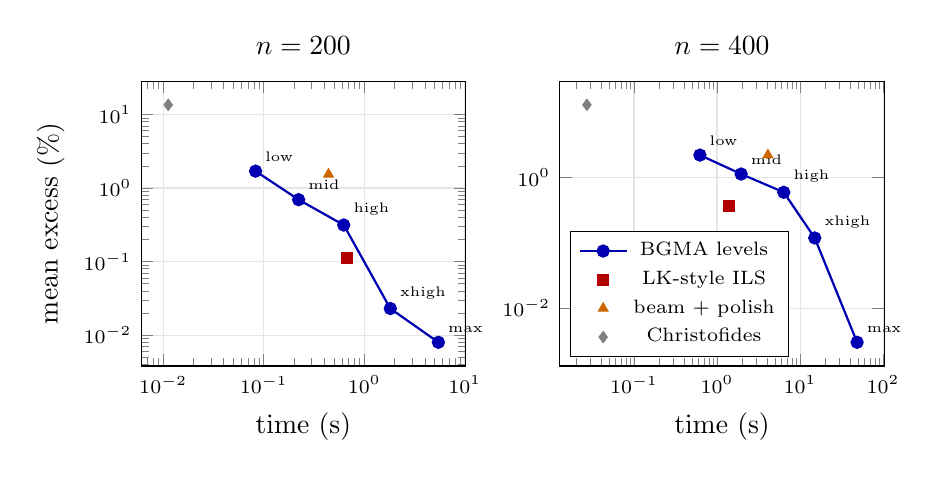
\begin{tikzpicture}
\begin{axis}[name=a0,width=0.47\textwidth,height=5.2cm,xmode=log,ymode=log,clip=false,title={$n=200$},xlabel={time (s)},ylabel={mean excess (\%)},grid=major,grid style={gray!20},legend style={font=\scriptsize,at={(0.03,0.03)},anchor=south west},tick label style={font=\scriptsize}]
\addplot[thick,mark=*,blue!70!black] coordinates {(0.08297,1.695) (0.2224,0.694) (0.6249,0.314) (1.815,0.023) (5.456,0.008)};
\node[font=\tiny,anchor=south west] at (axis cs:0.08297,1.695) {low};
\node[font=\tiny,anchor=south west] at (axis cs:0.2224,0.694) {mid};
\node[font=\tiny,anchor=south west] at (axis cs:0.6249,0.314) {high};
\node[font=\tiny,anchor=south west] at (axis cs:1.815,0.023) {xhigh};
\node[font=\tiny,anchor=south west] at (axis cs:5.456,0.008) {max};
\addplot[only marks,mark=square*,red!70!black] coordinates {(0.6718,0.111)};
\addplot[only marks,mark=triangle*,orange!80!black] coordinates {(0.4408,1.535)};
\addplot[only marks,mark=diamond*,gray] coordinates {(0.01123,13.486)};
\end{axis}
\begin{axis}[name=a1,at={(a0.east)},anchor=west,xshift=1.2cm,width=0.47\textwidth,height=5.2cm,xmode=log,ymode=log,clip=false,title={$n=400$},xlabel={time (s)},grid=major,grid style={gray!20},legend style={font=\scriptsize,at={(0.03,0.03)},anchor=south west},tick label style={font=\scriptsize}]
\addplot[thick,mark=*,blue!70!black] coordinates {(0.6224,2.215) (1.954,1.135) (6.367,0.596) (15.03,0.119) (48.63,0.003)};
\node[font=\tiny,anchor=south west] at (axis cs:0.6224,2.215) {low};
\node[font=\tiny,anchor=south west] at (axis cs:1.954,1.135) {mid};
\node[font=\tiny,anchor=south west] at (axis cs:6.367,0.596) {high};
\node[font=\tiny,anchor=south west] at (axis cs:15.03,0.119) {xhigh};
\node[font=\tiny,anchor=south west] at (axis cs:48.63,0.003) {max};
\addplot[only marks,mark=square*,red!70!black] coordinates {(1.405,0.371)};
\addplot[only marks,mark=triangle*,orange!80!black] coordinates {(4.104,2.221)};
\addplot[only marks,mark=diamond*,gray] coordinates {(0.02710,13.026)};
\legend{BGMA levels,LK-style ILS,beam + polish,Christofides}
\end{axis}
\end{tikzpicture}

\caption{Time against mean relative excess on the synthetic instances (log--log; excess floored at
0.003\% for plotting). BGMA levels are joined in order \lvl{low}$\to$\lvl{max}.}
\label{fig:curve}
\end{figure}

Five observations follow.

\emph{The dial works, at a steep price.} Each level costs about 2--3.5 times the previous one. The cost
ratios at $n=400$ are \val{ratios400}. Up to $n=400$ each level also cuts the remaining excess roughly in
half, from \rt{bgma-low}{400}{gap} at \lvl{low} to \rt{bgma-max}{400}{gap} at \lvl{max}. Fitted between
$n=20$ and $400$, time grows as about $n^{\val{expAll@bgma-low}}$ at \lvl{low} and
$n^{\val{expAll@bgma-max}}$ at \lvl{max}, but the growth steepens with $n$: between $100$ and $400$ the
exponents are \val{exp@bgma-low} and \val{exp@bgma-max}. This matches the cost model of
Section~\ref{sec:method}, in which the number of quadratic polishes itself grows with $n$. The
LK-style baseline grows as $n^{\val{exp@lkh}}$ over the same range.

\emph{From $n=200$ an LK-style ILS is the better trade-off below the top two levels.} At $n=200$ it
takes about as long as \lvl{high} (\rt{lkh}{200}{ms} against \rt{bgma-high}{200}{ms}) for about a
third of the excess (\rt{lkh}{200}{gap} against \rt{bgma-high}{200}{gap}). At $n=400$ the LK-style baseline takes
\rt{lkh}{400}{ms} for \rt{lkh}{400}{gap}. That beats \lvl{mid} (\rt{bgma-mid}{400}{ms}, \rt{bgma-mid}{400}{gap}) and \lvl{high}
(\rt{bgma-high}{400}{ms}, \rt{bgma-high}{400}{gap}) on both time and quality. \lvl{low} is faster
(\rt{bgma-low}{400}{ms}) but its excess is much larger (\rt{bgma-low}{400}{gap}). Only \lvl{xhigh} and \lvl{max} find shorter tours (\rt{bgma-xhigh}{400}{gap} and
\rt{bgma-max}{400}{gap}), and they need \val{xhighVsLk400} and \val{maxVsLk400} times the LK-style
baseline's time. At $n\le 100$ the picture reverses. Both methods are near-optimal, and BGMA's middle
levels get there faster (at $n=100$: \lvl{mid} \rt{bgma-mid}{100}{ms}, LK-style \rt{lkh}{100}{ms}).

\emph{The memetic stage earns its place over its predecessor.} The beam + polish pipeline reaches the
same quality as \lvl{low} at $n=400$ (\rt{tuned}{400}{gap} against \rt{bgma-low}{400}{gap}) but takes
\val{tunedVsLow400} times as long. Polishing every beam final is wasteful; polishing only the best
screened candidates is not.

\emph{The guarantee is far from typical behaviour.} Christofides runs in milliseconds and is
\val{chrRange} above the best found tour from $n=50$ up. From $n=50$ its
excess is \val{chrVsLow} times that of \lvl{low}.

\emph{Monotonicity across levels is not guaranteed.} Only the \lvl{max}~$\ge$~\lvl{xhigh} step is
monotone by construction (Section~\ref{sec:method}). On individual instances a cheaper level sometimes
beats a more expensive one; on rat783, for example, the \lvl{xhigh} unit beats both \lvl{max} restarts (Section~\ref{sec:tsplib}).

\subsection{TSPLIB: true gaps against published optima}\label{sec:tsplib}

Table~\ref{tab:tsplib} scores BGMA \lvl{max} and the LK-style baseline against the published optimum of
each instance. Distances are rounded as \code{EUC\_2D} prescribes. Instances up to $n=442$ were run
with ten seeds. The larger ones were run with one to three seeds, because one \lvl{max} run there costs
minutes to over an hour of CPU time. The \emph{equal-time} columns restart the LK-style search with new seeds until it has spent the median
serial cost of one BGMA \lvl{max} run on that instance. They report the best tour found within that
budget, the number of restarts it allowed, and the cumulative CPU time at which the restarts first
reached a tour at least as short as BGMA's median.


\begin{table*}[t]
\centering\scriptsize
\caption{TSPLIB \code{EUC\_2D} instances against published optima. Gaps are true gaps $L/L^\ast-1$.
``Serial time'' is the median CPU time of one \lvl{max} run (sum of its three units); with three worker
threads the wall clock is about a third of it. ``Below opt.''\ is how far the 600-iteration 1-tree bound
lies under the optimum, i.e.\ how much a bound gap would overstate the true gap.}
\label{tab:tsplib}
\setlength{\tabcolsep}{3pt}
\begin{tabular}{@{}lrrrrrrrrrrrrr@{}}
\toprule
 & & & \multicolumn{4}{c}{BGMA \lvl{max}} & \multicolumn{3}{c}{LK-style, one run} & \multicolumn{3}{c}{LK-style, equal time} & 1-tree\\
\cmidrule(lr){4-7}\cmidrule(lr){8-10}\cmidrule(lr){11-13}\cmidrule(l){14-14}
instance & $n$ & seeds & opt. & median & best & serial & opt. & median & time & best & runs & reached & below\\
 & & & hits & gap & gap & time & hits & gap & & gap & & median & opt.\\
\midrule
eil51 & 51 & 10 & 9/10 & 0.00\% & 0.00\% & 352\,ms & 1/10 & +0.23\% & 19\,ms & 0.00\% & 26 & 44\,ms & 0.82\%\\
berlin52 & 52 & 10 & 10/10 & 0.00\% & 0.00\% & 385\,ms & 10/10 & 0.00\% & 45\,ms & 0.00\% & 10 & 45\,ms & 0.00\%\\
st70 & 70 & 10 & 10/10 & 0.00\% & 0.00\% & 496\,ms & 8/10 & 0.00\% & 77\,ms & 0.00\% & 7 & 136\,ms & 0.59\%\\
kroA100 & 100 & 10 & 10/10 & 0.00\% & 0.00\% & 876\,ms & 10/10 & 0.00\% & 127\,ms & 0.00\% & 7 & 131\,ms & 1.62\%\\
pr124 & 124 & 10 & 10/10 & 0.00\% & 0.00\% & 1.44\,s & 8/10 & 0.00\% & 331\,ms & 0.00\% & 5 & 324\,ms & 1.63\%\\
bier127 & 127 & 10 & 10/10 & 0.00\% & 0.00\% & 1.58\,s & 3/10 & +0.83\% & 224\,ms & 0.00\% & 6 & 636\,ms & 0.72\%\\
ch130 & 130 & 10 & 10/10 & 0.00\% & 0.00\% & 1.68\,s & 3/10 & +0.29\% & 429\,ms & 0.00\% & 5 & 1.10\,s & 0.56\%\\
tsp225 & 225 & 10 & 10/10 & 0.00\% & 0.00\% & 7.75\,s & 3/10 & +0.37\% & 451\,ms & 0.00\% & 15 & 1.44\,s & 0.97\%\\
fl417 & 417 & 10 & 10/10 & 0.00\% & 0.00\% & 57.6\,s & 1/10 & +0.78\% & 3.05\,s & 0.00\% & 20 & 20.3\,s & 5.34\%\\
pcb442 & 442 & 10 & 0/10 & +0.66\% & +0.51\% & 64.8\,s & 0/10 & +0.56\% & 1.13\,s & +0.25\% & 60 & 1.18\,s & 0.56\%\\
u574 & 574 & 3 & 0/3 & +0.50\% & +0.33\% & 3.5\,min & 0/3 & +1.14\% & 3.23\,s & +0.47\% & 62 & 3.2\,min & 0.53\%\\
rat783 & 783 & 3 & 0/3 & +1.15\% & +1.04\% & 9.7\,min & 0/3 & +1.23\% & 1.74\,s & +0.69\% & 298 & 5.61\,s & 0.38\%\\
pr1002 & 1002 & 1 & 0/1 & +2.10\% & +2.10\% & 39.8\,min & 0/1 & +2.19\% & 5.73\,s & +1.07\% & 400 & 12.1\,s & 0.90\%\\
u1060 & 1060 & 1 & 0/1 & +1.45\% & +1.45\% & 58.4\,min & 0/1 & +2.06\% & 6.66\,s & +0.55\% & 555 & 12.8\,s & 0.86\%\\
\bottomrule
\end{tabular}

\end{table*}

\paragraph{Up to $n=442$.}
BGMA \lvl{max} returned the optimum in \val{tsSmallHits} of \val{tsSmallRuns} runs. It did so on all ten
seeds for \val{tsSmallAllSeeds} of the \val{tsSmallCount} instances and on nine seeds for eil51. It never
did on pcb442 (median \ts{pcb442}{maxMedGap}, best \ts{pcb442}{maxBestGap}). Single LK-style runs are
much less reliable: \val{tsSmallLkHits} of \val{tsSmallRuns} were optimal. They are also much cheaper,
and the best of ten LK-style runs reaches the optimum on \val{tsSmallLkAny} of the \val{tsSmallCount} instances, the same ones as BGMA. On fl417 the
ten LK-style runs together cost \ts{fl417}{lkTotal}, against \ts{fl417}{maxSerial} for one \lvl{max} run.
On pcb442 the LK-style baseline is better outright: a median of \ts{pcb442}{lkMedGap} in \ts{pcb442}{lkMs}
per run, against \ts{pcb442}{maxMedGap} for \lvl{max} in \ts{pcb442}{maxSerial}. Instance structure
matters as much as size. fl417, with its dense clusters, is solved on every seed, while pcb442, which
is only slightly larger, is solved on none.

\paragraph{Beyond $n=500$.}
The median gaps of \lvl{max} range from \val{tsBigRange}. These are true gaps: the excess is genuine tour excess,
not slack in a bound. The three portfolio units show the top of the dial flattening. On u574 the
\lvl{xhigh} unit reached \ts{u574}{armXhigh} and the two \lvl{max} restarts \ts{u574}{armMax}. On rat783
they reached \ts{rat783}{armXhigh} against \ts{rat783}{armMax}. On pr1002 they reached
\ts{pr1002}{armXhigh} against \ts{pr1002}{armMax}, and on u1060 \ts{u1060}{armXhigh} against
\ts{u1060}{armMax}. The heavier \lvl{max} configuration is not reliably better than \lvl{xhigh} on the
same instance. Its contribution is mostly that of extra independent samples. A single \lvl{max} run on
pr1002 costs \ts{pr1002}{maxSerial} of CPU time (\ts{pr1002}{maxWall} on three threads).

% filled when the equal-time data exist


\paragraph{The bound gap misleads.}
The last column of Table~\ref{tab:tsplib} shows the 1-tree bound \val{boundBelowRange} below the optimum,
depending on the instance. An optimal fl417 tour has a bound gap of \ts{fl417}{boundGap}, while an
optimal berlin52 tour has \ts{berlin52}{boundGap}. Had we reported bound gaps, as is common when no
optimum is known, fl417 would have looked like BGMA's worst instance. It is one of its best.

\subsection{Robustness, determinism and degenerate inputs}\label{sec:robust}
The stress harness ran \lvl{low} and \lvl{max} on seven families at $n=20$, $100$ and $400$
(\val{stressRuns} runs, Table~\ref{tab:stress}). Every tour was checked to be a valid permutation with
a correctly recomputed length. No run produced an invalid tour (\val{stressInvalid} failures), and no
tour came out shorter than the proven bound (\val{stressViolations} violations).

\begin{table}[t]
\centering\footnotesize
\caption{Degenerate and known-optimum families. ``Gap to bound'' is listed per $n$ ($20$, $100$, $400$)
and is a ceiling on the true gap. \emph{fine} and \emph{coarse} are the same point set scaled by
$10^{-3}$ and $10^{6}$.}
\label{tab:stress}
\setlength{\tabcolsep}{4pt}
\input{generated/stress_table}
\end{table}

\paragraph{Known optima by construction.}
For points in convex position the hull cycle is optimal, and both levels returned it at every size.
At $n=1000$, \lvl{low} returned \val{convex1000@low@hull} in \val{convex1000@low} and \lvl{max}
returned \val{convex1000@max@hull} in \val{convex1000@max} of CPU time. Collinear points (optimum: twice
the span) and coincident points (optimum: 0) were solved exactly. On the $20\times 20$ grid,
\lvl{max} met the 1-tree bound, which proves its tour optimal, while \lvl{low} did not.

\paragraph{The bound can be very loose.}
On collinear points the tour is optimal by construction, yet its bound gap reads
\val{stress@line@max@100} at $n=100$ and \val{stress@line@max@400} at $n=400$. A degree-constrained relaxation cannot express the structure of a line. This
is the same phenomenon as fl417 in Section~\ref{sec:tsplib}, in a more extreme form.

\paragraph{Scale dependence.}
The \emph{fine} and \emph{coarse} families are one point set at two scales, so a scale-free method
would return the same relative gap on both. \lvl{max} nearly does (\val{stress@fine@max@400} against \val{stress@coarse@max@400} at
$n=400$). \lvl{low} does not (\val{stress@fine@low@400} against \val{stress@coarse@low@400}), because the anneal temperature is set in absolute units (Section~\ref{sec:limits}).

\paragraph{Determinism.}
Every level was run three times on each of two $n=100$ instances (\val{repeatRuns} runs in
\val{repeatGroups} groups). In \val{repeatIdentical} of the \val{repeatGroups} groups the repeats
returned the same length and the same tour. Runs are a deterministic function of (instance, seed,
level), also under the worker pool.


\section{Discussion}\label{sec:discussion}

\paragraph{What the evidence supports.}
BGMA is exact on every instance small enough for Held--Karp. At \lvl{max} it returns the published
optimum on \val{tsSmallSomeSeed} of the \val{tsSmallCount} TSPLIB instances up to $n=442$, on nearly
every seed, and on none of the ten seeds of pcb442 (Table~\ref{tab:tsplib}). On the synthetic families its effort dial trades time for quality in a
regular way up to a few hundred cities. Beyond about 500 cities the residual is real tour excess of
\val{tsBigRange} (median over seeds), not an artefact of the bound, and the top of the ladder stops paying.

\paragraph{What it does not support.}
BGMA is not competitive with the state of the art. The clearest evidence is in this paper itself. An
LK-style iterated local search of a few hundred lines, in the same language, matches or beats BGMA's
lower levels at equal or lower cost (Section~\ref{sec:synthetic}). Real LK implementations are stronger
still: LKH~\citep{helsgaun2009} and EAX~\citep{nagata2013} find optimal or near-optimal tours on
instances of these sizes in seconds, and Concorde~\citep{applegate2006} proves optimality for all of
them. We did not run those codes, so we make no quantitative claim about them. A reader who needs good
TSP tours should use them. What BGMA adds is a small, readable, dependency-free implementation with
an explicit budget dial and a measurement record that can be reproduced end to end.

\paragraph{Why the top of the ladder stops paying.}
For $n\ge 80$, \lvl{xhigh} and \lvl{max} use the same beam width ($n/2$) and the same number of
generations ($n/8$). What \lvl{max} adds is more islands, a larger pool, more final polishing and a
second restart, and it pays for all of it in full. With ERX, a 2-opt/Or-opt polish and weak
perturbation, more of the same search mostly revisits the same basins. A stronger local search
(Or-3opt, LK) inside the memetic loop, or a recombination that preserves more structure (EAX), is the
likely lever, not more budget.

\paragraph{The 1-tree bound is a poor yardstick for heuristics.}
The bound gap over-states the true gap by an amount that depends on the instance, not on the tour.
On fl417 an optimal tour reads as \ts{fl417}{boundGap} above the bound, on berlin52 as \ts{berlin52}{boundGap}, and on collinear points an
optimal tour reads \val{stress@line@max@400} above the bound (Section~\ref{sec:robust}). Two heuristics compared through bound gaps on
different instances are therefore not compared at all. Wherever a true optimum is available it should
be used.

\section{Limitations and threats to validity}\label{sec:limits}

\begin{itemize}\itemsep2pt
\item \emph{In-sample tuning.} The ladder was tuned on the synthetic families of
Section~\ref{sec:synthetic}. TSPLIB was held out, but there are only fourteen instances, chosen as
standard \code{EUC\_2D} benchmarks of increasing size and not at random.
\item \emph{Seeds.} TSPLIB instances up to $n=442$ use ten seeds. Larger instances use one to three,
because a single \lvl{max} run there costs \ts{u574}{maxSerial} to \ts{u1060}{maxSerial} of CPU time. Their gaps are a few
observations, not distributions.
\item \emph{One machine, one runtime.} All times come from one laptop and one Node.js version. Ratios
between methods in the same harness are more portable than absolute times.
\item \emph{Baselines.} The LK-style baseline is ours and simpler than LKH. It runs at its default
budget, so it is not time-matched to the upper BGMA levels. Its ten-seed best is still far cheaper than
one \lvl{max} run.
\item \emph{Scale dependence.} The anneal temperature $T_0=\max(1,0.02n)$ is in absolute distance
units. On instances with very large or very small coordinates the anneal degenerates into greedy
descent or a random walk (it returns the best tour it saw, so it cannot make a child worse). The other
operators are scale-free. Normalising $T_0$ by the mean candidate edge length is the obvious fix and
has not been done.
\item \emph{Synthetic optima.} Above $n=22$ the synthetic families have no known optimum. For them
we report only relative excess and the bound gap, which is a ceiling.
\end{itemize}

\section{Conclusion}\label{sec:conclusion}

BGMA is a compact memetic heuristic with an explicit effort dial. Measured against known optima it is
exact on small instances, reliably optimal at its top level on most TSPLIB instances up to a few
hundred cities, and \val{tsBigRange} above the optimum (median over seeds) from 574 to 1060 cities. The dial is regular up
to 400 cities and flattens beyond. The same measurements show its limits plainly. An LK-style iterated
local search of comparable size, restarted for the same CPU time, matches or beats BGMA's top level on
every TSPLIB instance tested. Mature solvers are in a different class. We release the implementation,
the harnesses and every data file behind this paper, so that each number can be regenerated with one
script. The most promising change is to replace the 2-opt/Or-opt polish with LK moves, i.e.\ to make
BGMA a memetic algorithm over LK local optima in the manner of \citet{merz2001}, and to normalise the
annealing scale. Whether the memetic layer then adds anything over plain restarts is the open question.

\section*{Reproducibility}
Code, data and this paper's sources are at \url{https://github.com/Mhmdrza/bgma} (MIT
licence). \code{paper/verify.sh} reruns every experiment; TSPLIB files must be obtained separately.
\code{paper/gen\_tables.js} regenerates every table and number from \code{paper/data/}, and
Appendix~\ref{app:repro} lists the commands. Each TSPLIB result file stores the tour, so the reported
lengths can be checked independently.

\section*{Acknowledgements}
Parts of the implementation, the experiment harnesses and the text were developed with the help of an
AI coding assistant (Anthropic's Claude). All experiments were run by the author, and the author is
responsible for the content.



\bibliographystyle{plainnat}
\bibliography{refs}

\appendix
\section{Reproduction}\label{app:repro}
With Node.js $\ge 18$ and no other dependency:
{\footnotesize
\begin{verbatim}
npm test                                  # self-tests
TSPLIB=/path/to/tsplib sh paper/verify.sh # all experiments
node paper/gen_tables.js                  # data -> tables
\end{verbatim}
}
The steps of \code{verify.sh} can be run separately (\code{sh paper/verify.sh C} runs only the
ten-seed TSPLIB step). Individual runs:
{\footnotesize
\begin{verbatim}
node tuning/validate_effort.js --ns=18,20 --seeds=5
node bench/runtime_bench.js --json=runtime.json --md=1
node tuning/tsplib_bench.js --file=pcb442.tsp --opt=50778 \
     --levels=lk,max --seed=1 --jobs=3
node tuning/stress_parallel.js --ns=400 --families=convex,line,grid --levels=low,max
node src/hybrid/hybrid_effort.js --n=200 --effort=max --bound=1
\end{verbatim}
}
Runs are deterministic given (instance, seed, level): repeating a command reproduces the tour exactly,
and only the times vary.


\end{document}
